\chapter{Implementation}\label{sec:implementation}


This section describes the reference implementation for the conceptual framework in Chapter \ref{sec:concept}.
First, the general architecture is explained.
Various components and interaction techniques of the geographical visualization are detailed.
The integration of the geographical visualization in the existing \visan{} is shown.
The connection of the conceptual framework and the implemented framework is examined.

\section{Implemented interactions}

In the course of this thesis the following interactions have been implemented:
\begin{itemize}
  \item
    Select

    \begin{itemize}
      \item
        Highlighting an entity is possible by moving the mouse cursor on a geographic feature in the \gv{} or a block in the \tmap{}.
        The corresponding block or geographic feature will be highlighted respectively.
      \item
        A click on a block in the \tmap{} selects this entity in the \gv{} and vice versa.
      \item
        Holding the control key, multiple clicks on a block in the \tmap{} creates a group of selected entities.
        Corresponding geographic feature or blocks in the \tmap{} or \gv{} are selected as well.
    \end{itemize}

  \item
    Explore

    \begin{itemize}
      \item Selecting a block in the \tmap{} centers the viewpoint in the \gv{} on the corresponding geographic feature.
      \item Selecting a group of blocks in the \tmap{} centers the viewpoint in the \gv{} on the boundaries of all corresponding geographic features.
    \end{itemize}

  \item
    Reconfigure

    \begin{itemize}
      \item
        Choosing a different data set updates the geometries in the \gv{}.
      \item
        Selecting another shape for the \tmap{} (e.g. point instead of polygon geometries) changes the visual representation in the \gv{}.
    \end{itemize}

  % \item
  %   \emph{Filter}: The user double-clicks on a region in a geographical map and the \tmap{} will be based on data of only that region.
\end{itemize}
\todo[inline]{If we still have time, add filter interaction here}

\section{Coordinated Multiple View Layout}

Figure~\ref{fig:implementation:layout} shows the layout of the different views from the user perspective.
The \tmap{} is on the left, the \gv{} is on the right and some additional views to inspect and manually publish messages are displayed.

The currently visualized data set is called ``Wahlkreise'' and consists of German administrative districts.
The \tmap{} is tiled based on unemployment rate and the colour is based on the percentage of high-school graduates.
District ``Magdeburg'' is selected in the \gv{} with an unusually high percentage of graduates compared to other districts with a similar unemployment rate.

\begin{figure}[ht]
  \centering
  \caption{%
    This Figure shows the layout of the \cmv{}, red lines indicate the borders of different views.
  }\label{fig:implementation:layout}
  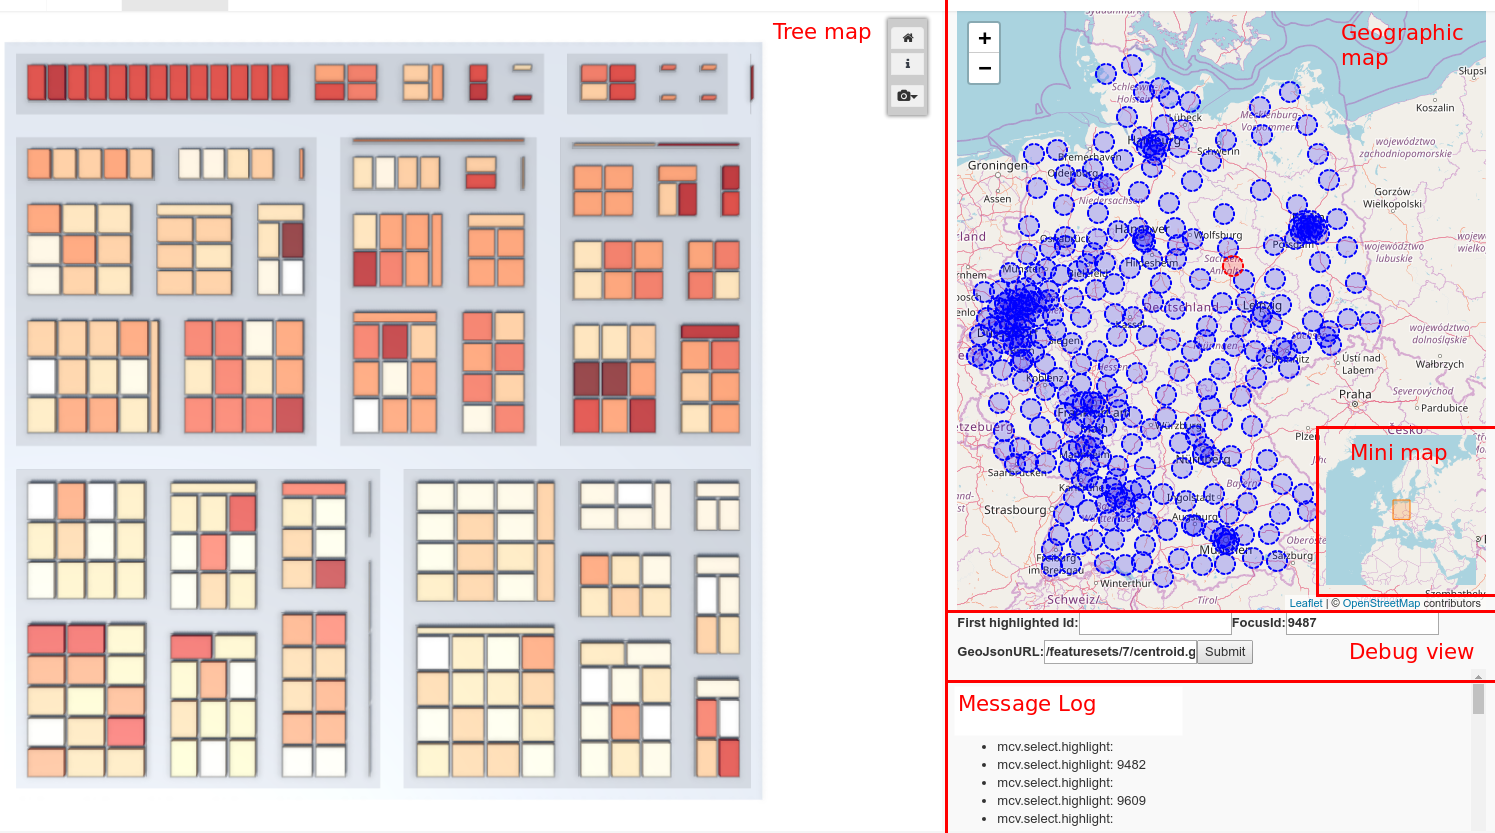
\includegraphics[width=\textwidth]{figures/implementation/Layout}
\end{figure}


\section{Architecture}
The architecture of the implementation is depicted in the class diagram in Figure~\ref{fig:implementation:architecture}.
For each of the views in Figure~\ref{fig:implementation:layout} you can see a corresponding class in Figure~\ref{fig:implementation:architecture}, i.e.\ \attr{Treemap}, \attr{MapComponent}, \attr{MessageLog} and \attr{DebugView}.

All views have a reference to \attr{MultiviewCoordinator} in order to subscribe to interactions.
The rendering \tmap{} is controlled by \attr{UAController}, thus it is connected to \attr{MultiviewCoordinator} through this class.
The \attr{MultiviewCoordinator} itself does not have a visual representation.

\subsection{Update mechanisms}
In Figure~\ref{fig:implementation:architecture} views with a \attr{render} are implemented as React components and can be rendered in place of a node inside the DOM tree.
React components and their dependant components get automatically re-rendered if their internal state changes.

E.g. if the position of the view point of the \attr{MapComponent} changes, that will re-render the included \attr{Map} which depends on the position.
If the Geometries of the visualized data set are updated, that will change the \attr{GeoJSON} component but not the \attr{Map}.

% Views implemented with React are dependency free except for a reference to a \attr{MultiviewCoordinator}.
% This makes those classes very easy to test.


\begin{figure}[ht]
  \centering
  \caption{%
    Architecture of components.
    Every class with a \attr{render} method is a React component.
    \attr{MultiviewCoordinator} is used to coordinate \tmap{} and \gv{} as well as to load geometry data.
  }\label{fig:implementation:architecture}
  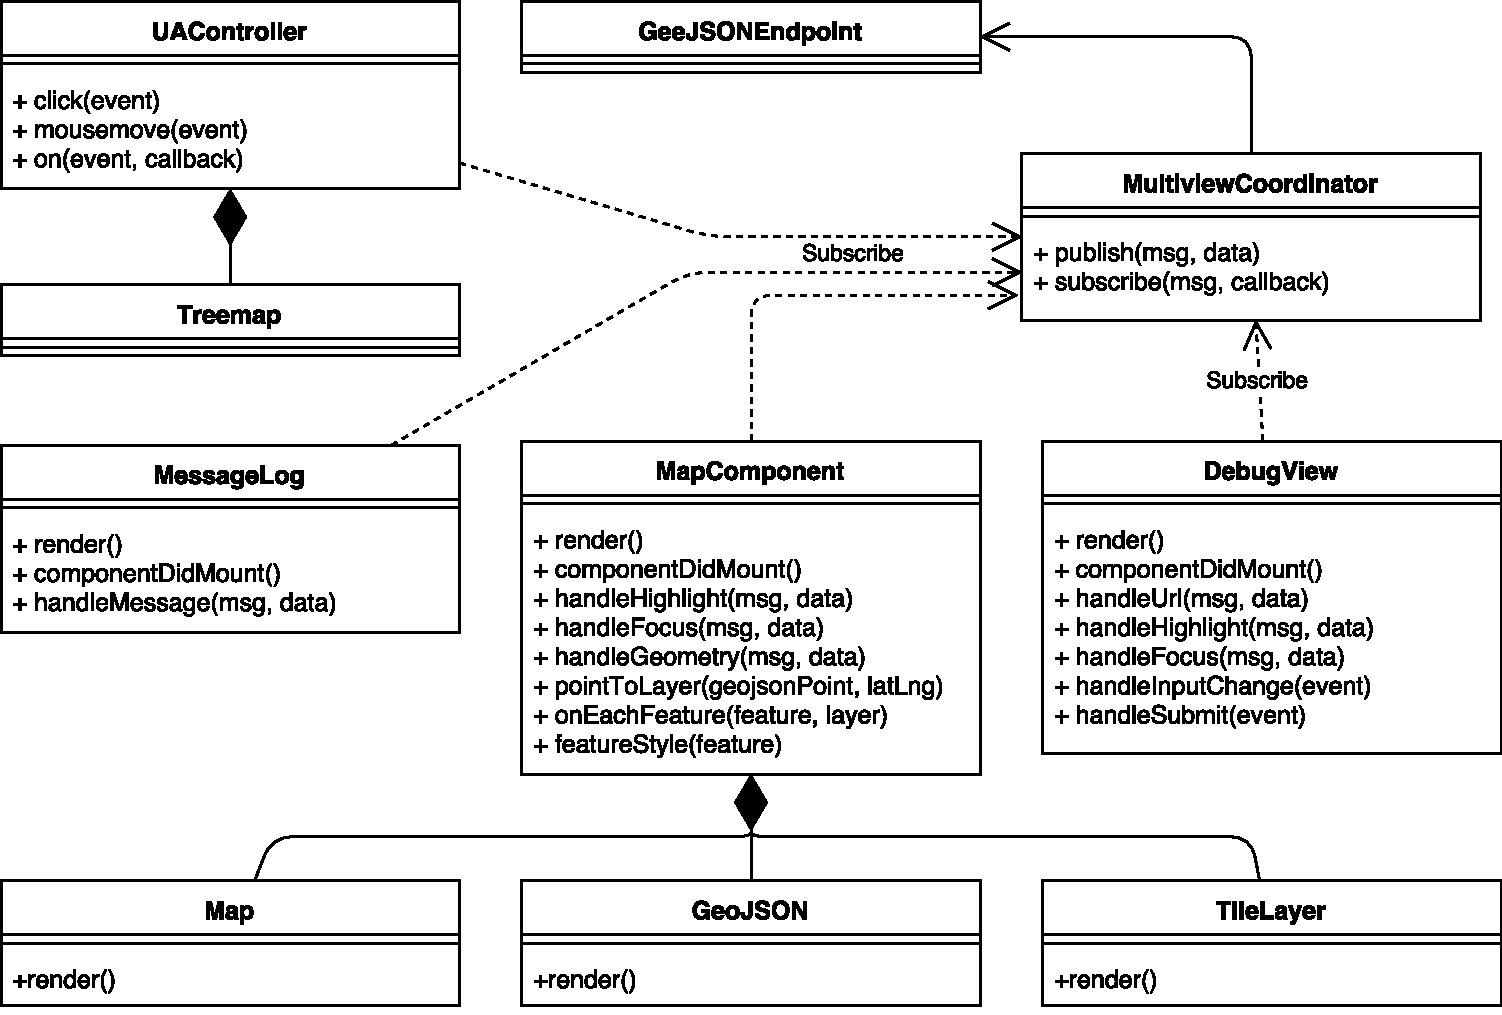
\includegraphics[width=\textwidth]{figures/implementation/Architecture.pdf}
\end{figure}

\section{Notifications}

The automatic update mechanism works only within the virtual DOM of React components.
Updates on view level need to be implemented manually.

In accordance to Chapter~\ref{sec:concept}, the class \attr{MultiviewCoordinator} implements the \attr{publish-subscribe} pattern for coordination and works as a broker for interactions across \cmvs{}.
To achieve this, it uses the JavaScript library \attr{PubSubJS} which is an topic-based, asynchronous implementation of the pattern.

Let's take an example from a common usage scenario:
During initialization, all views subscribe to \attr{MultiviewCoordinator} in order to re-render after interactions.
Then the user chooses another data set and the geometries are updated.
After that, the user clicks with the mouse on a geographic feature and the corresponding item is focused.
You can see this scenario in the sequence diagram in Figure~\ref{fig:implementation:sequence-diagram}.

\begin{figure}[ht]
  \centering
  \caption{%
    This sequence diagram shows the notification of different components during a common usage scenario.
  }\label{fig:implementation:sequence-diagram}
  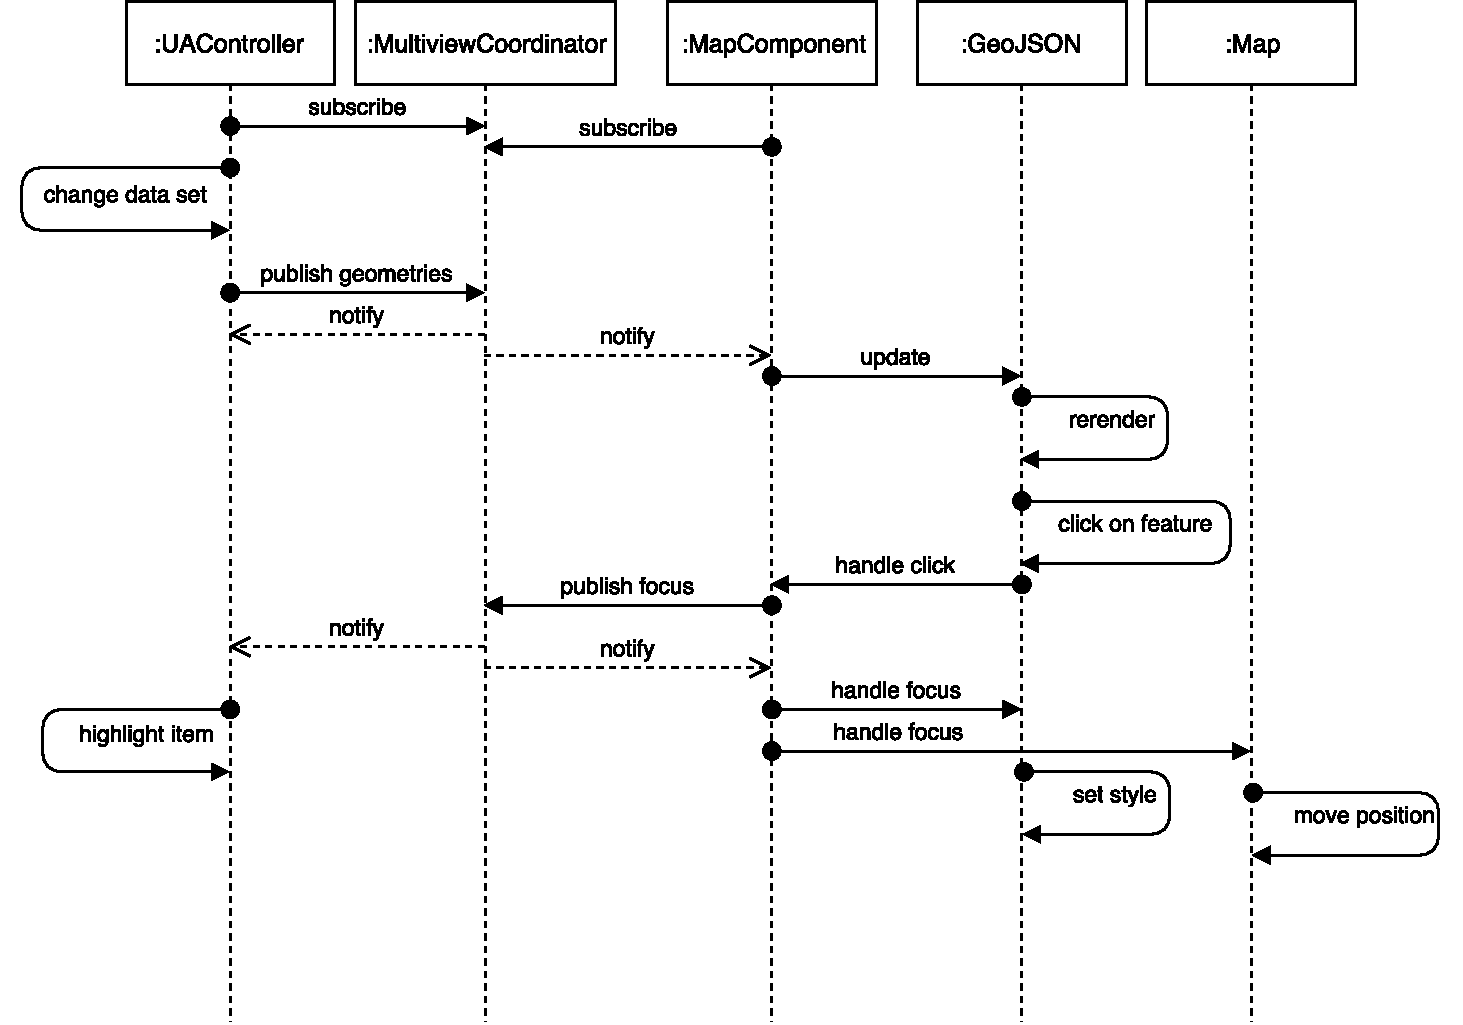
\includegraphics[width=\textwidth]{figures/implementation/SequenceDiagram}
\end{figure}


\subsection{Encoding of interaction category and purpose}
Each view gets a reference to the coordinator, e.g. during initialization, and can subscribe to interactions as seen in Listing~\ref{lst:implementation:subscribe}.

\attr{PubSubJS} allows nested topics, so categories and purposes are encoded as nested strings.
A view can subscribe to a group of interactions, e.g.\ the group \attr{mcv.select} includes both \attr{mcv.select.highlight} and \attr{mcv.select.focus}.
This approach gives each view self-responsibility of the implementation of individual interactions.

According to Chapter~\ref{sec:concept}, categories and purposes are encoded with nested strings.
Figure~\ref{fig:implementation:encoding} gives an example of a select interaction with the purpose to focus on three entities.

\begin{figure}[ht]
  \centering
  \caption{%
    Example of the encoding of interaction category and purpose.
  }\label{fig:implementation:encoding}
  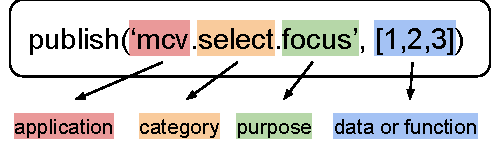
\includegraphics[width=\textwidth]{figures/implementation/Encoding}
\end{figure}

Not only basic data types like numbers and strings can be published, as seen in Listing~\ref{lst:implementation:subscribe}, but also functions.
If an interaction of type \attr{filter} is published, it is not necessary to publish all filtered ids of entities explicitly.
Instead, the \attr{data} of the interaction can be a threshold function which, applied on an entity, returns whether or not the entity is filtered.

\lstinputlisting[
  label={lst:implementation:subscribe},
  caption={
    A simplified example how to subscribe to an interaction.
  }
]{listings/implementation/subscribe.js}


\section{MultiviewCoordinator}

As a central part of the implementation, the \attr{MultiviewCoordinator} is also used for certain performance optimizations and data integrity considerations.
Therefore, it is responsible to query geometry data.

Geometries are exchanged with \attr{GeoJSON}\footnotemark as data format.
\footnotetext{
  GeoJSON is a format for encoding a variety of geographic data structures~\parencite{GeoJSON2017}.
  Based on JSON, it can represent simple geographic features like points, lines and areas and reserves a properties object for non-spatial attributes.
}

If the user selects a different data set, the \attr{url} of the GeoJSON endpoint changes and an update of the geometry data is required.
This behaviour is implemented by the \attr{MultiviewCoordinator} which observes all changes to the \attr{url} of the GeoJSON endpoint.
If the \attr{url} changes, the coordinator fetches geometry data, publishes a change of the geometries and all subscribed views can re-render.
This is also a performance optimization, as it reduces the number of requests to the \attr{GeoJSON} endpoint.

An example of these geometries can be seen in listing~\ref{lst:geojson:example}.
For convenience, the file includes the aggregated data in the \attr{properties} of each feature.
In this case the colors the shapes of the \tmap{} are based on the value of \attr{user_count_normalized}.
Each feature comes with a unique \attr{id} which is published when a user interacts with the feature.

\lstinputlisting[
  label={lst:geojson:example},
  caption={
    A GeoJSON example of a user distribution across German federal states.
    Coordinates are omitted.
  }
]{listings/implementation/example.geojson}

\section{Render views in the DOM}

Adding the \gv{} to the DOM is straightforward.
Listing~\ref{lst:implementation:dom} shows an example how to use React's low-level API to render components inside the DOM.
It uses a HTML id \attr{multiview-map-component} to reference a particular node in the HTML document.
The HTML document needs to import three JavaScript files, i.e.\ two imported libraries required by React and the compiled JavaScript application.

\lstinputlisting[
  label={lst:implementation:dom},
  lastline=12,
  caption={
    Example application written in TypeScript.
    Views can be added to the DOM individually.
    The implementation exposes convenient TypeScript declarations, here \attr{MultiviewCoordinator} and \attr{MapComponent} are imported.
  }
]{listings/implementation/dom.tsx}

The reference implementation of the conceptual framework is written in \attr{TypeScript}\footnotemark.
The implementation exports typescript declaration and you can see an import of the classes \attr{MapComponent} and \attr{MultiviewCoordinator} on lines 1 to 3 in Listing~\ref{lst:implementation:dom}.
\footnotetext{
  TypeScript is a typed superset of JavaScript that compiles to plain JavaScript.
  It provides optional static typing, classes and interfaces and helps to reduce errors by raising type errors at compile time.
}


% \section{Software patterns}\label{sec:implementation:patterns}

% \textbf{The Observer pattern} allows multiple \emph{observers} to react to changes of an observed state.
% In our case, the observed state is the \attr{MultiviewCoordinator}.
% Any change to the \attr{MultiviewCoordinator} will subsequently be broadcasted to all connected views.


% \textbf{Publisher subscriber}
% In our particular case we apply a special form of the observer pattern, the so called ``Publish-subscribe'' pattern\parencite{Eugster2003}.
% Publish-subscribe is a messaging pattern which is widely used in message queues.
% In this scenario, senders of messages simply categorize their messages which will be consumed by subscribers of the category.
% The scenario has very low coupling, publishers do not even need to know the existence of subscribers.

% \textbf{Component pattern}
% State-of-the-art JavaScript component frameworks like ReactJS and EmberJS follow the component pattern for the architecture of a single page web application.
% The component pattern imposes a hierarchical structure on a website.
% Each component is responsible for a task and may contain other components.
% The components are joined at the root node of the page.

% This pattern is very applicable to \cmvs{}.
% The different views of \cmvs{} share state, i.e.\ the feature, that is currently highlighted or the applied filter on the data.
% So the views are components and their closest common ancestor is the \cmv{} itself, controlling state and passing user interaction down to it's children.

% \textbf{Actions up --- Data down}

% Version 2.0 of Ember introduced a common phrase how to use this pattern effectively: ``Data down, actions up''\parencite{Emberigniter2017}
% In the domain of \cmvs{} actions would mean user interactions, e.g.\ a click on a feature.
% The action will notify the controlling \cmv{} component.
% Actions may change data, and the changes will be passed to to all dependent views.
% These views are then re-rendered.

% Examples for the kind of data that might trigger a re-rendering of a view:
% \begin{itemize}
%   \item
%     The selected feature or a list of selected features
%   \item
%     A list of thresholds for certain features as a filter
% \end{itemize}


\section{Map Component}

The geographical visualization makes use of three components of the React Leaflet library:
\attr{Map}, \attr{TileLayer} and \attr{GeoJSON}.
Listing \ref{lst:implementation:render} shows the \attr{render} method of the component.

\lstinputlisting[
  label={lst:implementation:render},
  caption={\attr{render} method of the Map component of the geographical visualization.}
]{listings/implementation/render.tsx}

The \attr{render} method is the only required method of a React component.
It will be invoked on the initial rendering of the component of the \attr{DOM} and on every update of the component's properties.
React's templating language ``\attr{JSX}'' allows to nest other child components into the React parent component.
In this case the \attr{Map} component includes a \attr{TileLayer} \attr{GeoJSON} component from the \attr{react-leaflet} library.
This library conveniently provides ``React components for Leaflet maps.''~\parencite{ReactLeaflet2017}.

\subsection{GeoJSON Component}

The \attr{GeoJSON} component is provided by the \attr{Map} component with a couple of properties:
It gets a
\begin{enumerate*}[label=(\arabic*)]
  \item
    geojsonURL as well as a
  \item
    geojson as data attribute. Furthermore a couple of callbacks is passed into the child component, including
  \item
    featureStyle,
  \item
    pointToLayer and
  \item
    onEachFeature.
\end{enumerate*}

This way, the parent \attr{Map} component controls the data flow and without a \attr{geojson} object, no polygons are placed on the map.
A changed \attr{geojsonURL} will always update the child component as it is used a \attr{key} on the \attr{GeoJSON} component.
The callbacks passed into the \attr{GeoJSON} component control the visual representation of each polygon and they add event handlers for a mouse click or a mouse move on each polygon.
Listing \ref{lst:implementation:onEachFeature} shows the event handlers added to the map.

\lstinputlisting[
  label={lst:implementation:onEachFeature},
  caption={\attr{onEachFeature} callback, adding handlers for mouse events.}
]{listings/implementation/onEachFeature.tsx}

First we cache all layers in the internal state of the \attr{Map} component.
On each \attr{mouseover} event, the \attr{id} of the feature is published as \attr{mcv.select.highlight} interaction.
A \attr{click} event is distinguished if the control key is pressed or not.
In the latter case, the id of the feature is either added or removed from the list of focused ids and then the list of focused ids is published as \attr{mcv.select.focus} interaction.

\lstinputlisting[
  label={lst:implementation:featureStyle},
  caption={\attr{featureStyle} callback, configuring the visual appearance depending on the currently highlighted or focused feature ids.}
]{listings/implementation/featureStyle.tsx}

The \attr{featureStyle} in Listing \ref{lst:implementation:featureStyle} method is very straightforward.
If the feature is currently focused, the \attr{fillColor} of the polygon is red, otherwise blue.
Likewise, if the feature is currently highlighted, the polygon has a white, solid stroke.

\lstinputlisting[
  label={lst:implementation:pointToLayer},
  caption={\attr{pointToLayer} callback, if a feature of \attr{GeoJSON} has a point geometry, it will be shown as a circle.}
]{listings/implementation/pointToLayer.tsx}

Finally, we configure how to display point geometries in callback \attr{poinToLayer}.
Since normal markers do not have a configurable color and style, we instruct the \attr{GeoJSON} component to render a \attr{CircleMarker} for each point geometry instead.
This way, the same options of \attr{featureStyle} can be applied to both point and area geometries.




